\documentclass[aspectratio=169,11pt]{beamer}
% Shared Beamer setup for Ms Economía PEG, Problem Set 1, Team 3.
\usepackage[T1]{fontenc}
\usepackage[utf8]{inputenc}
\usepackage[spanish,es-noshorthands]{babel}
\usepackage{booktabs}
\usepackage{graphicx}
\usepackage{amsmath,amssymb}
\usepackage{tabularx}
\usepackage{xcolor}
\usepackage{tikz}
\usepackage{hyperref}

\graphicspath{{../02_outputs/figures/}{img/}{./}}
\newcommand{\nsample}{14,761}
\newcommand{\ntrain}{10,260}
\newcommand{\nvalid}{4,501}
\newcommand{\sharefemale}{47.3}
\newcommand{\medianincome}{992,745}
\newcommand{\meanincome}{1,617,237}
\newcommand{\medianhours}{48}
\newcommand{\meanage}{38.9}
\newcommand{\peakuncond}{40.6}
\newcommand{\peakuncondlo}{40.1}
\newcommand{\peakuncondhi}{41.2}
\newcommand{\peakcond}{43.6}
\newcommand{\peakcondlo}{42.8}
\newcommand{\peakcondhi}{44.5}
\newcommand{\rtwoageu}{0.050}
\newcommand{\rtwoagec}{0.226}
\newcommand{\gapuncond}{-21.2}
\newcommand{\gaphc}{-27.2}
\newcommand{\gappref}{-19.6}
\newcommand{\gapjob}{-18.9}
\newcommand{\gapcoef}{-0.218}
\newcommand{\gapse}{0.012}
\newcommand{\gapseboot}{0.012}
\newcommand{\fwlcoef}{-0.218}
\newcommand{\peakmen}{50.5}
\newcommand{\peakmenlo}{49.1}
\newcommand{\peakmenhi}{52.3}
\newcommand{\peakwomen}{45.6}
\newcommand{\peakwomenlo}{44.4}
\newcommand{\peakwomenhi}{47.0}
\newcommand{\bestmodel}{P6: Flexible age, education, and hours}
\newcommand{\bestshort}{P6: polinomio flexible}
\newcommand{\gapuncondabs}{21.2}
\newcommand{\gaphcabs}{27.2}
\newcommand{\gapprefabs}{19.6}
\newcommand{\bestvalid}{0.6160}
\newcommand{\bestloocv}{0.5825}
\newcommand{\besttrain}{0.5797}
\newcommand{\topvar}{Socioeconomic stratum}
\newcommand{\topdelta}{0.1185}


\definecolor{navy}{HTML}{1B365D}
\definecolor{accent}{HTML}{B85C38}
\definecolor{slate}{HTML}{5B6B73}
\definecolor{gold}{HTML}{C4A35A}
\definecolor{ice}{HTML}{F4F6F8}

\setbeamercolor{structure}{fg=navy}
\setbeamercolor{frametitle}{fg=navy,bg=white}
\setbeamercolor{title}{fg=navy}
\setbeamercolor{subtitle}{fg=slate}
\setbeamercolor{author}{fg=slate}
\setbeamercolor{institute}{fg=slate}
\setbeamercolor{date}{fg=slate}
\setbeamercolor{item}{fg=accent}
\setbeamercolor{footline}{fg=slate}
\setbeamercolor{normal text}{fg=navy}

\setbeamertemplate{navigation symbols}{}
\setbeamertemplate{itemize items}[circle]
\setbeamerfont{frametitle}{series=\bfseries,size=\large}
\setbeamerfont{title}{series=\bfseries,size=\LARGE}

% Escudo Uniandes: portada y esquina superior derecha de cada diapositiva.
\newcommand{\uniandeslogo}[1][0.92cm]{
\includegraphics[height=#1]{logo_uniandes.png}}

\setbeamertemplate{frametitle}{%
  \nointerlineskip
  \vspace{0.18cm}%
  \leavevmode
  \hbox to \textwidth{%
    \begin{minipage}[c]{0.88\textwidth}
      \raggedright
      \usebeamerfont{frametitle}\usebeamercolor[fg]{frametitle}\insertframetitle
    \end{minipage}%
    \hfil
    \raisebox{-0.12cm}{\uniandeslogo[0.72cm]}%
  }%
  \vspace{0.12cm}%
}

\setbeamertemplate{title page}{%
  \vbox{}
  \vspace{0.15cm}
  \begin{flushright}
    \uniandeslogo[1.15cm]
    \hspace{0.08cm}
  \end{flushright}
  \vspace{0.55cm}
  \begin{center}
    {\usebeamerfont{title}\usebeamercolor[fg]{title}\inserttitle\par}
    \vspace{0.45em}
    {\usebeamerfont{subtitle}\usebeamercolor[fg]{subtitle}\insertsubtitle\par}
    \vspace{1.15em}
    {\usebeamerfont{author}\insertauthor\par}
    \vspace{0.55em}
    {\usebeamerfont{institute}\insertinstitute\par}
    \vspace{0.85em}
    {\usebeamerfont{date}\insertdate\par}
  \end{center}
}

\setbeamertemplate{footline}{
  \leavevmode%
  \hbox{%
    \begin{beamercolorbox}[wd=.55\paperwidth,ht=2.4ex,dp=1.2ex,leftskip=1em]{footline}
      \tiny Grupo 3 $\cdot$ Ms Economía PEG $\cdot$ Universidad de los Andes
    \end{beamercolorbox}%
    \begin{beamercolorbox}[wd=.45\paperwidth,ht=2.4ex,dp=1.2ex,rightskip=1em,right]{footline}
      \tiny \insertframenumber/\inserttotalframenumber
    \end{beamercolorbox}}%
  \vskip0pt%
}

\newcommand{\statblock}[3]{%
  \begin{tikzpicture}
    \node[fill=ice, inner sep=10pt, text width=0.42\textwidth, align=center] {
      {\fontsize{20}{24}\selectfont\bfseries\color{navy} #1}\\[4pt]
      {\small\color{slate} #2}\\[2pt]
      {\scriptsize\color{accent} #3}
    };
  \end{tikzpicture}%
}

\newcommand{\source}[1]{\vfill{\scriptsize\color{slate} #1}}


\title{Brecha de g\'enero en ingreso laboral}
\subtitle{Problem Set 1 $\cdot$ Secci\'on 2}
\author{Juli\'an Herrera \and Andr\'es Silva \and Valentina Vera}
\institute{Ms Economía PEG $\cdot$ Big Data and Machine Learning para Econom\'ia Aplicada\\ Universidad de los Andes}
\date{2026-20 $\cdot$ Grupo 3}

\begin{document}

\begin{frame}[plain]
  \titlepage
\end{frame}

\begin{frame}{Result overview}
  \vspace{0.3em}
  \begin{columns}[T]
    \column{0.5\textwidth}
      \statblock{\gapuncondabs\%}{menos ingreso (mujeres)}{brecha incondicional}
    \column{0.5\textwidth}
      \statblock{\gapprefabs\%}{brecha preferida}{edad, educaci\'on, horas y relab}
  \end{columns}
  \vspace{0.9em}
  Capital humano \textbf{ampl\'ia} la brecha (de \gapuncondabs\% a \gaphcabs\%): las mujeres de la muestra son, en promedio, m\'as educadas, as\'i que no controlar educaci\'on subestima $\beta$.
  Horas y tipo de ocupaci\'on la comprimen hasta \gapprefabs\%. Esa ca\'ida s\'i puede ser un bad control.
  Picos: hombres \peakmen\ (IC [\peakmenlo, \peakmenhi]); mujeres \peakwomen\ (IC [\peakwomenlo, \peakwomenhi]).
  \source{Coeficiente preferido $=\gapcoef$ (EE anal\'itico $\gapse$; EE bootstrap FWL $\gapseboot$). $N=\nsample$.}
\end{frame}

\begin{frame}{Pregunta y decisi\'on metodol\'ogica}
  \begin{block}{La elecci\'on de controles es el resultado de esta secci\'on}
    ¿Cu\'anto de la brecha sobrevive cuando condicionamos en caracter\'isticas que una autoridad tributaria observa, y cu\'ales de esas caracter\'isticas no deber\'iamos condicionar si el objeto es la brecha \emph{causal}?
  \end{block}
  \vspace{0.5em}
  \begin{itemize}
    \item \textbf{Buenos controles:} edad y educaci\'on. Est\'an (en gran parte) determinadas antes del salario corriente.
    \item \textbf{Controles discutibles:} horas y \texttt{relab}. Pueden ser el canal de la brecha (selecci\'on a tiempo parcial, segregaci\'on ocupacional).
    \item \textbf{Malos controles claros:} formalidad y tama\~no de firma, si el inter\'es es discriminaci\'on. \'Utiles si el inter\'es es predicci\'on.
  \end{itemize}
\end{frame}

\begin{frame}{La brecha no es un artefacto de un solo nivel educativo}
  \begin{center}
    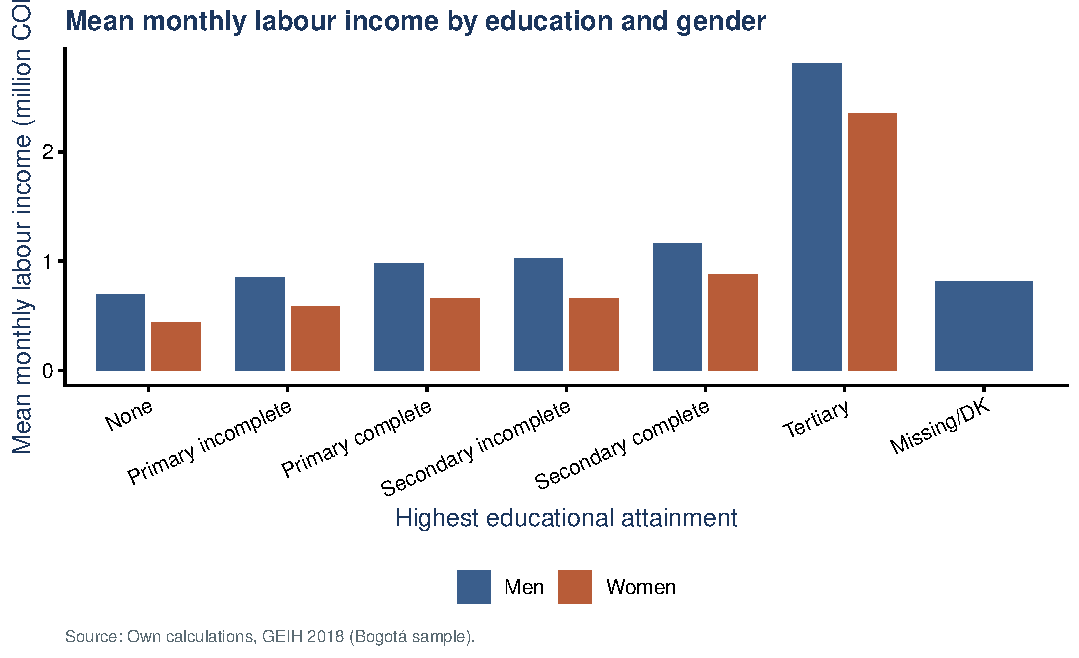
\includegraphics[width=0.92\textwidth]{fig_gap_by_education.pdf}
  \end{center}
\end{frame}

\begin{frame}{Especificaciones}
  \begin{align*}
    \log(w_i) &= \alpha + \beta \, \mathrm{Mujer}_i + u_i \\[2pt]
    \log(w_i) &= \alpha + \beta \, \mathrm{Mujer}_i + f(\mathrm{Edad}_i) + \gamma' \mathrm{Educ}_i + u_i \\[2pt]
    \log(w_i) &= \alpha + \beta \, \mathrm{Mujer}_i + f(\mathrm{Edad}_i) + \gamma' \mathrm{Educ}_i + \theta \, \mathrm{Horas}_i + \delta' \mathrm{Relab}_i + u_i
  \end{align*}
  \vspace{0.2em}
  \begin{itemize}
    \item $\beta$ se reporta tambi\'en como $100(e^{\beta}-1)$: diferencia porcentual aproximada.
    \item Especificaci\'on preferida: capital humano \emph{m\'as} horas y \texttt{relab}. Es la m\'as \'util para fiscalizaci\'on; no es la m\'as limpia para causalidad.
    \item FWL: el mismo $\beta$ se obtiene residualizando $\log(w)$ y $\mathrm{Mujer}$ respecto a los controles.
  \end{itemize}
\end{frame}

\begin{frame}{La brecha se comprime, no desaparece}
  \begin{center}
    \footnotesize
    \resizebox{0.98\textwidth}{!}{\begin{tabular}{lcccccc}
\toprule
Specification & Female coef. & Analytical SE & Bootstrap SE & Gap (\%) & R$^2$ & N \\
\midrule
M1: Unconditional & -0.238 & 0.015 & 0.015 & -21.2 & 0.018 & 14,761 \\
M2: + Age & -0.257 & 0.014 & 0.015 & -22.7 & 0.070 & 14,761 \\
M3: + Stratum & -0.287 & 0.013 & 0.013 & -24.9 & 0.267 & 14,761 \\
M4: + Education & -0.320 & 0.012 & 0.013 & -27.4 & 0.346 & 14,761 \\
M5: + Formality & -0.301 & 0.011 & 0.012 & -26.0 & 0.445 & 14,761 \\
M6: + Hours/Occupation (preferred) & -0.199 & 0.011 & 0.011 & -18.1 & 0.535 & 14,761 \\
\bottomrule
\end{tabular}
}
  \end{center}
  \source{EE bootstrap solo en la especificaci\'on preferida, v\'ia FWL. El resto usa EE anal\'iticos OLS.}
\end{frame}

\begin{frame}{FWL recupera el mismo coeficiente}
  \begin{center}
    \footnotesize
    \resizebox{0.98\textwidth}{!}{\begin{tabular}{ccccc}
\toprule
OLS female coefficient & FWL coefficient & Analytical SE & FWL bootstrap SE & Absolute difference \\
\midrule
-0.199116 & -0.199116 & 0.011 & 0.011 & 0.00000000 \\
\bottomrule
\end{tabular}
}
  \end{center}
  \vspace{0.7em}
  \begin{itemize}
    \item FWL no cambia la interpretaci\'on: $\beta$ sigue siendo la diferencia en log ingreso \emph{dentro} de la variaci\'on de ``mujer'' que no es linealmente explicada por los controles.
    \item El EE bootstrap es un chequeo de infencia, no un estimador distinto.
    \item Si FWL y OLS no coincidieran, habr\'ia un error de implementaci\'on. Coinciden.
  \end{itemize}
\end{frame}

\begin{frame}{Perfiles por g\'enero, especificaci\'on preferida}
  \begin{center}
    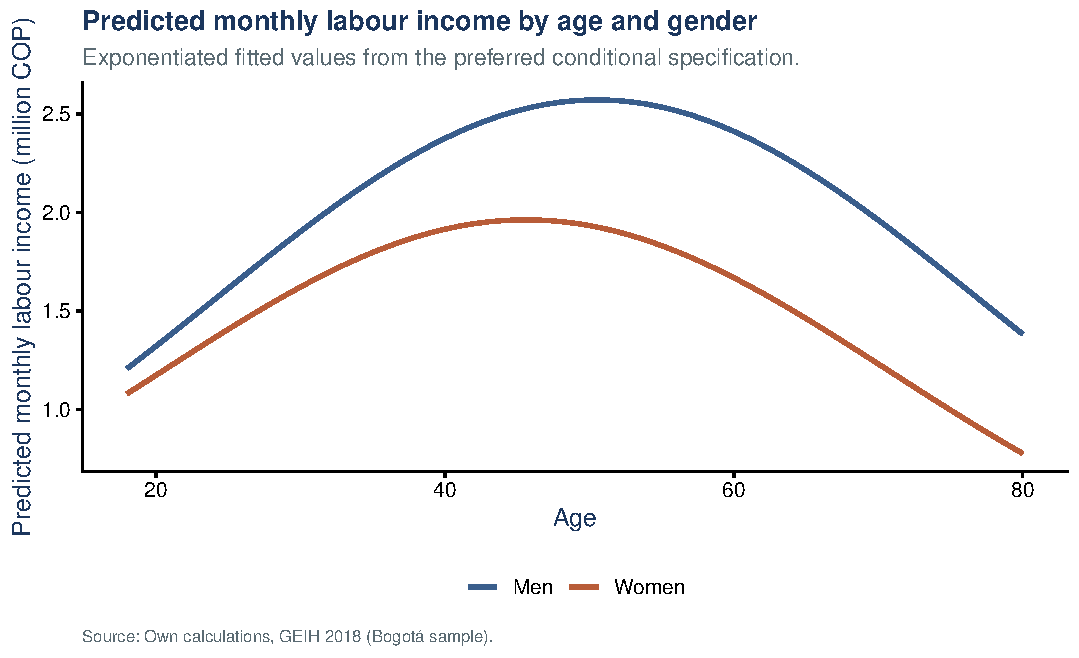
\includegraphics[width=0.92\textwidth]{fig_gap_profiles_cop.pdf}
  \end{center}
\end{frame}

\begin{frame}{Lectura}
  \begin{itemize}
    \item Una autoridad que ignore el g\'enero va a \textbf{sobrepredecir} el ingreso de las mujeres y marcarlas como subdeclarantes con m\'as frecuencia. Eso no es neutral.
    \item Una autoridad que condicione en ocupaci\'on ``explica'' parte de la brecha con segregaci\'on. Para auditor\'ia puede ser correcto; para equidad, no.
    \item Los picos distintos (\peakmen\ vs.\ \peakwomen) implican que el ciclo de vida no es el mismo. Un perfil \'unico por edad es una mala regla para ambos grupos.
  \end{itemize}
  \vspace{0.5em}
  \begin{block}{Takeaway}
    La brecha incondicional es \gapuncondabs\%. Condicionar en educaci\'on la sube a \gaphcabs\% (efecto supresor). Con horas y tipo de ocupaci\'on queda en \gapprefabs\%. El n\'umero del informe depende de si el objeto es causalidad o predicci\'on. Nosotros reportamos la secuencia y usamos la especificaci\'on preferida para la DIAN.
  \end{block}
\end{frame}

\end{document}
